% ============================================================
%  BAB 3 – PEMBAHASAN
% ============================================================


\chapter*{PEMBAHASAN}
\refstepcounter{chapter}
\addcontentsline{toc}{chapter}{PEMBAHASAN}
\pdfbookmark[0]{PEMBAHASAN}{pembahasan}

\section{Judul Subbagian Pertama}

% Uraian tahapan kegiatan penelitian – kalimat informasi (bukan kalimat perintah)
Tahapan pertama yang dilakukan dalam penelitian ini adalah \ldots\ldots\ldots\ldots
\ldots\ldots\ldots\ldots\ldots\ldots\ldots\ldots\ldots\ldots\ldots\ldots\ldots\ldots

% Contoh penyertaan gambar
\begin{figure}[H]
  \centering
  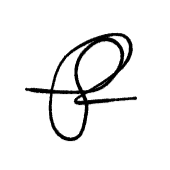
\includegraphics[width=0.8\textwidth]{gambar/gambar-31}
  \caption{Keterangan Gambar 3.1}
  \label{fig:gambar31}
\end{figure}

Seperti yang ditunjukkan pada Gambar~\ref{fig:gambar31}, \ldots\ldots\ldots\ldots\ldots

\section{Judul Subbagian Kedua}

\ldots\ldots\ldots\ldots\ldots\ldots\ldots\ldots\ldots\ldots\ldots\ldots\ldots\ldots

\subsection{Judul Sub-Subbagian Pertama}

\ldots\ldots\ldots\ldots\ldots\ldots\ldots\ldots\ldots\ldots\ldots\ldots\ldots\ldots

\subsection{Judul Sub-Subbagian Kedua}

\ldots\ldots\ldots\ldots\ldots\ldots\ldots\ldots\ldots\ldots\ldots\ldots\ldots\ldots

\section{Hasil}

Hasil yang diperoleh dari penelitian ini adalah \ldots\ldots\ldots\ldots\ldots\ldots
\ldots\ldots\ldots\ldots\ldots\ldots\ldots\ldots\ldots\ldots\ldots\ldots\ldots\ldots

% Contoh tabel hasil
\begin{table}[H]
  \centering
  \caption{Hasil Pengujian}
  \label{tab:hasil}
  \begin{tabular}{|c|l|c|c|}
    \hline
    No. & Skenario Uji & Hasil yang Diharapkan & Hasil Aktual \\
    \hline
    1   & Skenario 1  & Berhasil              & Berhasil     \\
    2   & Skenario 2  & Berhasil              & Berhasil     \\
    \hline
  \end{tabular}
\end{table}

Berdasarkan Tabel~\ref{tab:hasil}, \ldots\ldots\ldots\ldots\ldots\ldots\ldots\ldots
